\question{Механизм создания инверсной населенности уровней в четырехуровневой системе. Способы накачки}

\begin{figure}[h]
\begin{center}
    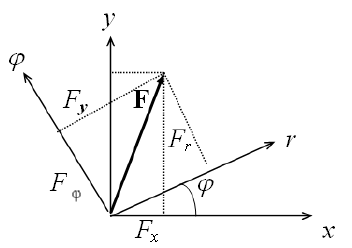
\includegraphics[width=.47\textwidth]{11_1}
\end{center}
\end{figure}

Для 4 уровневой системы необходимо, чтобы 3 и 1 уровни быстро расселялись, а
переход частиц в возбуждённое состояние \( (0\to3) \) происходил быстрее, чем
процесс излучения \( (2\to1) \). Отсюда можно получить условия для вероятностей:
\begin{gather*}
    S_{32}\gg W_{30},\\
    S_{10}\gg W_{21},\\
    W_{03} > A_{21}.
\end{gather*}
Очевидно, что для работы этой схемы уже нет необходимости в возбуждении большого
числа частиц, так как нижним лазерным уровнем является вспомогательный
быстрорасселяемый уровень, число частиц на котором мало.
